%\documentclass[handout,xcolor=x11names,compress,10pt]{beamer}
\documentclass[xcolor=x11names,compress,10pt]{beamer}
%% General document %%%%%%%%%%%%%%%%%%%%%%%%%%%%%%%%%%

\usepackage{../tslides}

%\usepackage{alltt}
%\usepackage{xcolor}
%\usepackage{float}
%\usepackage{graphicx,wrapfig}
%\usepackage{multirow}
%\usepackage{tabularx,colortbl}
%\usepackage{listings}  
%\usepackage{multicol}  
%\usepackage{hyperref}  
%
%\newcommand{\intens}[1] {{\color{DeepSkyBlue3} #1}}
%\newcommand{\myalert}[1] {{\color{MedianOrange} #1}}
%

 
%=========================================

\begin{document}
\title{\\Curs 8}
\author{Fundamentele limbajelor de programare} 
\date{2020-2021} 

\frame{\titlepage} 

\frame{\frametitle{Cuprins}\tableofcontents} 


%-------------------------------------------------------------

%-------------------------------------------------------------
\section{Programare logică \& Prolog} \sectionframe
%-------------------------------------------------------------


%%-------------------------------------------------------------
%\begin{frame}{Logica matematică}
%
%\medskip
%\begin{columns}
%\begin{column}{.64\textwidth}
%\begin{itemize}	
%	\item Un mijloc de a clarifica/modela procesul de a "raționa".
%	\medskip
%	\item \intens{Logica ne permite să reprezentăm/modelăm probleme.}
%	\medskip 
%	\item Care logică?
%	\begin{itemize}
%	\item propozițională
%	\item de ordinul I
%	\item de ordin înalt
%	\item logici modale
%	\item logici temporale
%	\item logici cu mai multe valori
%	\item $\ldots$
%\end{itemize}
%\end{itemize}
%\end{column}
%\begin{column}{.3\textwidth}
%\vspace{-.5cm}
%\hspace{-1.2cm}
\includegraphics[scale=0.3]{img/Logic}
%\end{column}
%\end{columns}
%
%\medskip \pause
%\begin{center}
%{\color{red} Veți vedea cum poate fi folosită logica \\ în programare și în verificarea programelor.}
%\end{center}
%
%\end{frame}
%
%
%
%
%
%%---------------------------------------------------------------------
%
%%\begin{frame}{La acest curs vom folosi litere grecești!}
%
%%\medskip
%%\begin{figure}[h]
% % \centering
% %   \includegraphics[width=0.5\textwidth]{img/logos}
%%\end{figure}
%%\end{frame}
%
%
%
%
%
%
%%-------------------------------------------------------------
%\begin{frame}{Principalele paradigme de programare}
%\begin{itemize}
%	\item \intens{Imperativă} (\intens{\underline{cum}} calculăm)
%	\vspace{.2cm}
%	\begin{itemize}
%	\item \intens{Procedurală}
%		\vspace{.2cm}
%	\item \intens{Orientată pe obiecte}
%	
%	\end{itemize}
%	
%	\vspace{.5cm}
%	\item  \intens{Declarativă} (\intens{\underline{ce}} calculăm)
%		\vspace{.2cm}
%	\begin{itemize}
%	
%	\item \intens{Logică}
%	\vspace{.2cm}
%	\item \intens{Funcțională}
%	
%	\end{itemize}
%
%\end{itemize}
%
% \pause
%\begin{center}
%{\color{red} În continuare veți invăța \\  programare logică.}
%\end{center}
%\end{frame}
%
%%-------------------------------------------------------------
%%
%%\begin{frame}{Programare declarativă}
%%
%%	\begin{itemize}
%%		\item Programatorul spune \intens{ce} vrea să calculeze, dar nu specifică concret \intens{cum} calculează.
%%		\medskip
%%		\item Este treaba interpretorului (compilator/implementare) să identifice cum să efectueze calculul respectiv.
%%		\medskip
%%		\item \intens{Programarea logică} este un tip de programare declarativă!
%%		\medskip
%%		\item Tipuri de programare declarativă:
%%		\begin{itemize}
%%			\item Programare logică (e.g., Prolog)
%%			%\item limbaje de baze de date (SQL)
%%			\item Programare funcțională (e.g., Haskell)
%%			
%%		\end{itemize}
%%	\end{itemize}
%%
%%\end{frame}

%-------------------------------------------------------------
\begin{frame}{Programare logică}


\begin{itemize}
	\item \intens{Programarea logică} este o paradigmă de programare \\
	bazată pe logică formală.
	
	\vspace{.2cm} \pause
	\item Unul din sloganurile programării logice:
	\begin{center}
	\href{https://www.doc.ic.ac.uk/~rak/papers/History.pdf}{\intens{\textbf{Program = Logică + Control}}}  \quad {\em (R. Kowalski)}	
	\end{center} 
	
	\vspace{.2cm} \pause
	\item Programarea logică poate fi privită ca o deducție controlată.	
	
	\vspace{.2cm} \pause
	\item Un \intens{program} scris într-un limbaj de programare logică este
	\begin{center}
	\intens{o listă de formule într-o logică}
	\end{center}
	ce exprimă fapte și reguli despre o problemă.

	\vspace{.2cm} \pause
	\item Exemple de limbaje de programare logică: 
		\begin{itemize}
			\item \intens{Prolog}
			\item \intens{Answer set programming (ASP)}
			\item \intens{Datalog}
		\end{itemize}
\end{itemize}
\end{frame}

%---------------------------------------------------------------------

\begin{frame}{Ce veți vedea la laborator}
\medskip 

 \intens{Prolog}
\begin{itemize}
	\item bazat pe logica clauzelor Horn
	\item semantica operațională este bazată pe rezoluție
	\item este Turing complet
	\item vom folosi implementarea \intens{SWI-Prolog}
%	\item vom folosi varianta online \intens{SWISH} a SWI-Prolog
%	\begin{itemize}
%		\item \underline{\url{http://swish.swi-prolog.org/}}
%	\end{itemize}
\end{itemize}
\pause\medskip

\begin{block}{}
Limbajul Prolog este folosit pentru programarea sistemului IBM Watson!
\begin{center}

\includegraphics[scale=0.05]{img/watson}
\end{center}
Puteți citi mai multe detalii   \href{https://www.cs.nmsu.edu/ALP/2011/03/natural-language-processing-with-prolog-in-the-ibm-watson-system/}{\intens{aici}}.
\end{block}

\underline{Learn Prolog Now!\url{http://www.let.rug.nl/bos/lpn/}}
\end{frame}



%---------------------------------------------------------------------
%\begin{frame}
%\vspace{1cm}
%\begin{figure}[h]
 % \centering
 %   
\includegraphics[width=0.6\textwidth]{img/work}
%\end{figure}
%\end{frame}






%---------------------------------------------------------------------
\begin{frame}{Programare logică - în mod idealist}
\begin{itemize}
	\item Un \intens{"program logic"} este o colecție de proprietăți presupuse (sub formă de formule logice) despre lume (sau mai degrabă despre lumea programului).
	\medskip
	\item Programatorul furnizează și o proprietate (o formula logică) care poate să fie sau nu adevărată în lumea respectivă (\intens{întrebare, {\em query}}).
	\medskip
	\item Sistemul determină dacă proprietatea aflată sub semnul întrebării este o consecință a proprietăților presupuse în program.
	\medskip
		\item Programatorul nu specifică metoda prin care sistemul verifică dacă întrebarea este sau nu consecință a programului.
\end{itemize}
\end{frame}
%---------------------------------------------------------------------

%---------------------------------------------------------------------
%\begin{frame}{Programare logică - în mod idealist}
%\intens{Aspecte declarative} ale programării logice:
%\begin{itemize}
%	\item Programatorul nu specifică metoda prin care sistemul %verifică dacă întrebarea este sau nu consecință a %programului.
%	\medskip
%	\item Faptul că întrebarea chiar este sau nu consecinț%ă este independent de metoda aleasă de sistem.
%\end{itemize}
%\end{frame}
%---------------------------------------------------------------------



%---------------------------------------------------------------------
\begin{frame}{Exemplu de program logic}
\begin{center}
\begin{tabular}{rcl}
\texttt{oslo} & $\to$ & \texttt{windy} \\[.5em]
\texttt{oslo} & $\to$ & \texttt{norway} \\[.5em]
\texttt{norway} & $\to$ & \texttt{cold} \\[.5em]
\texttt{cold $\wedge$ windy} & $\to$ & \texttt{winterIsComing} \\[.5em]
& & \texttt{oslo}\\
\end{tabular}
\end{center}
\bigskip\pause

\begin{block}{Exemplu de întrebare}
\begin{center}
Este adevărat \intens{\texttt{winterIsComing}}?
\end{center}
\end{block}
\end{frame}
%---------------------------------------------------------------------

%---------------------------------------------------------------------
%\begin{frame}{Exemplu de întrebare}

%\begin{center}
%Este adevărat \intens{\texttt{winterIsComing}}?
%\end{center}

%\medskip
%\begin{figure}[h]
%  \centering
%    
\includegraphics[width=0.6\textwidth]{img/winter}
%\end{figure}

%\end{frame}

%---------------------------------------------------------------------
\begin{frame}{Putem să testăm în SWI-Prolog}
\intens{Program:}
\begin{alltt}
windy :- oslo. \\
norway :- oslo. \\
cold :- norway. \\
winterIsComing :- windy, cold. \\
oslo. \\
\end{alltt}

\bigskip
\intens{Intrebare:}
\begin{alltt}
?- winterIsComing.\\
true
\end{alltt}

\bigskip
\underline{\url{http://swish.swi-prolog.org/}}
\end{frame}
%---------------------------------------------------------------------
%---------------------------------------------------------------------
\begin{frame}{Sintaxă: constante, variabile, termeni compuși}

\bigskip

\begin{itemize}
	
		
		  \item \intens{Atomi}: \texttt{sansa, 'Jon Snow', 
		  jon\_snow}
		  \bigskip
		  \item \intens{Numere}: \texttt{23, 23.03,-1}
		
		\medskip
		
		\intens{Atomii} și \intens{numerele} sunt \intens{constante}.
		\medskip
		\item \intens{Variabile}: \texttt{X, Stark, \_house}

		\bigskip
			\item Termeni \intens{compuși}: \texttt{father(eddard, jon\_snow)},
			
\hspace*{1cm}\texttt{and(son(bran,eddard), daughter(arya,eddard))}

\begin{itemize}
\item[-]   forma generală:	\intens{atom(termen,$\ldots$, termen)}
 \item[-]  atom-ul care denumește termenul se numește \intens{functor}		      	
			      	
\item[-] numărul de argumente se numește \intens{aritate}			      	\end{itemize}
\end{itemize}

\begin{center}
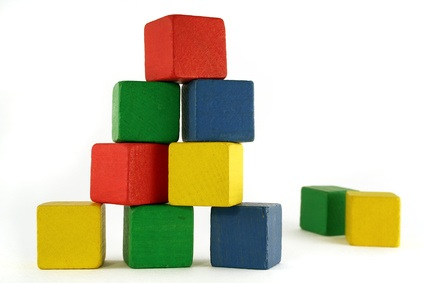
\includegraphics[scale=.2]{img/building-blocks}
\end{center}
\end{frame}


%---------------------------------------------------------------------
\begin{frame}{Un mic exercițiu sintactic}

Care din următoarele șiruri de caractere sunt \intens{constante} și care sunt \intens{variabile} în Prolog?

\begin{itemize}
	\item vINCENT \onslide<2->{-- \intens{constantă}}
	\item Footmassage \onslide<2->{-- \myalert{variabilă}} 
	\item variable23 \onslide<2->{-- \intens{constantă}}
	\item Variable2000 \onslide<2->{-- \myalert{variabilă}} 
	\item big\_kahuna\_burger \onslide<2->{-- \intens{constantă}}
	\item 'big  kahuna  burger' \onslide<2->{-- \intens{constantă}}
	\item big  kahuna  burger \onslide<2->{-- \alert{nici una, nici alta}}
	\item 'Jules' \onslide<2->{-- \intens{constantă}}
	\item \_Jules \onslide<2->{-- \myalert{variabilă}} 
	\item '\_Jules' \onslide<2->{-- \intens{constantă}}
\end{itemize}

\end{frame}

%---------------------------------------------------------------------
\begin{frame}[fragile]{Program în Prolog = bază de cunoștințe}

\begin{example}
Un program în Prolog:
\begin{columns}
\begin{column}{.5\textwidth}
\begin{verbatim}
father(eddard,sansa). 
father(eddard,jon_snow).

mother(catelyn,sansa). 
mother(wylla,jon_snow).

stark(eddard).
stark(catelyn).

stark(X) :- father(Y,X),  stark(Y).
\end{verbatim}
\end{column}
\begin{column}{.3\textwidth}

\includegraphics[scale=.8]{img/Stark.png}
\end{column}
\end{columns}
\smallskip
\end{example}
\medskip

Un program în Prolog este o \intens{bază de cunoștințe} (\intens{K}nowledge \intens{B}ase).
\end{frame}

%---------------------------------------------------------------------

\begin{frame}[fragile]{Program în Prolog = mulțime de predicate}

Practic, gândim un program în Prolog ca o mulțime de \intens{predicate}  cu ajutorul cărora descriem {\it lumea} ({\it universul}) programului respectiv.
 
\begin{example}
\begin{columns}
\begin{column}{.5\textwidth}
\begin{verbatim}
father(eddard,sansa). 
father(eddard,jon_snow).

mother(catelyn,sansa). 
mother(wylla,jon_snow).

stark(eddard).
stark(catelyn).

stark(X) :- father(Y,X),  stark(Y).
\end{verbatim}
\end{column}
\begin{column}{.3\textwidth}
\intens{\textbf{Predicate:}}\\
\intens{father/2}\\
\intens{mother/2}\\
\intens{stark/1}
\end{column}
\end{columns}
\smallskip
\end{example}



\end{frame}
%----------------------------------------------------


\begin{frame}{Un program în Prolog}

\begin{center}
%Un program în Prolog răspunde la întrebări.

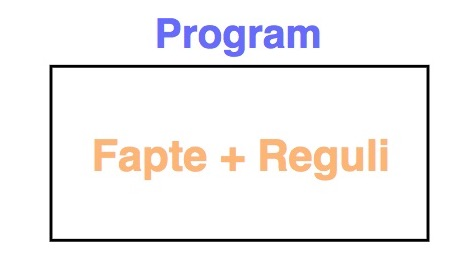
\includegraphics[scale=.3]{img/Prolog1}


\end{center}


\end{frame}
%---------------------------------------------------------------------


%---------------------------------------------------------------------
\begin{frame}{Program }

\begin{itemize}
	\item Un \intens{program} în Prolog este format din \intens{reguli} de forma
	\begin{center}
	\intens{\texttt{Head :- Body.}}
	\end{center} 
	\medskip
	
\item \intens{Head} este un predicat, iar \intens{Body} este o secvență de predicate separate prin virgulă.

\medskip
	
\item Regulile fără \texttt{Body} se numesc \intens{fapte}.
\end{itemize}

\medskip \pause
\begin{example}
\begin{itemize}
	\item  Exemplu de regulă: \texttt{stark(X) :- father(Y,X), stark(Y).}
	\item  Exemplu de fapt: \texttt{father(eddard, jon\_snow)}.
\end{itemize}
\end{example}
\end{frame}
%---------------------------------------------------------------------


\begin{frame}{Interpretarea din punctul de vedere al logicii}
\vspace*{0.3cm}

\begin{itemize}
\item operatorul \intens{\textbf{:-}} este implicația logică
 \intens{$\leftarrow$}
\begin{example}
\texttt{winterfell(X) :- stark(X)}
\smallskip

\intens{dacă} \texttt{stark(X)} \intens{este adevărat, atunci} 
\texttt{winterfell(X)} \intens{este adevărat.}
\end{example}
\pause

\item virgula \intens{,} este conjuncția \intens{$\wedge$}

\begin{example}
\texttt{stark(X) :- father(Y,X), stark(Y)}

\smallskip

\intens{dacă} \texttt{father(Y,X)} \intens{și} \texttt{stark(Y)}  \intens{sunt adevărate,}

\intens{atunci} \texttt{stark(X)} \intens{este adev\u rat.}
\end{example}
\end{itemize}
\end{frame}

\begin{frame}{Interpretarea din punctul de vedere al logicii}
\begin{itemize}
\item  mai multe reguli cu \intens{același \texttt{Head}} definesc același predicat, între defiții fiind un \intens{sau} logic. 
\end{itemize}

\begin{example}
\begin{alltt}
got\_house(X) :- stark(X).\\
got\_house(X) :- lannister(X).\\
got\_house(X) :- targaryen(X).\\
got\_house(X) :- baratheon(X).
\end{alltt}
\smallskip

\intens{dacă} 

 \texttt{stark(X)} \intens{este adevărat sau}
\texttt{lannister(X)} \intens{este adevărat sau}
 
  \texttt{targaryen(X)} \intens{este adevărat sau}
 \texttt{baratheon(X)}  \intens{este adevărat,}
  
\intens{ atunci} 

\texttt{got\_house(X)} \intens{este adevărat}.



\end{example}
\end{frame}

%---------------------------------------------------------------------

\begin{frame}{Un program în Prolog}

\begin{center}
%Un program în Prolog răspunde la întrebări.

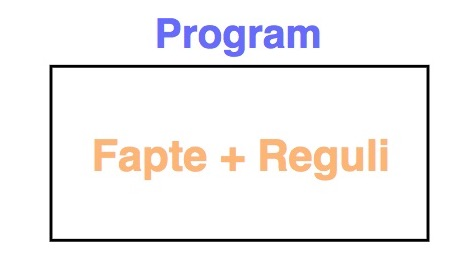
\includegraphics[scale=.3]{img/Prolog1}

\vspace*{1cm}

Cum folosim un program în Prolog?
\end{center}


\end{frame}
%---------------------------------------------------------------------

\begin{frame}{\^Intrebări în Prolog}

\begin{center}
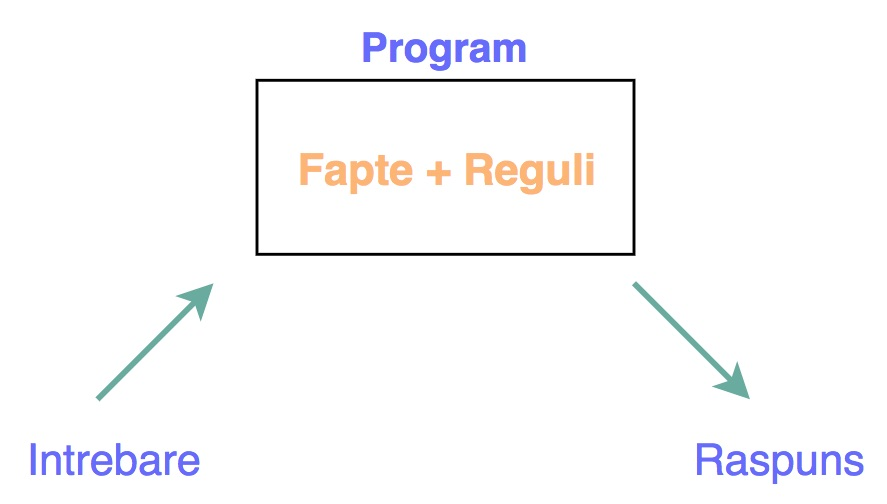
\includegraphics[scale=.3]{img/Prolog}
\end{center}

\end{frame}
%---------------------------------------------------------------------

%---------------------------------------------------------------------

\begin{frame}{\^Intrebări și ținte în Prolog}

\begin{itemize}
	\item Prolog poate răspunde la întrebări legate de consecințele relațiilor descrise într-un program în Prolog.
	\smallskip
	\item \intens{\^Intrebările} sunt de forma:
	\begin{center}
	\intens{\texttt{?- predicat$_1$($\ldots$),$\ldots$,predicat$_n$($\ldots$).}}
	\end{center}
	\smallskip
	\item Prolog verifică dacă întrebarea este o consecință a relațiilor definite în program.
	\smallskip
	\item Dacă este cazul, Prolog caută valori pentru variabilele care apar în întrebare astfel încât întrebarea să fie o consecință a relațiilor din program.
\smallskip	
	\item un predicat care este analizat pentru a se răspunde la o întrebare se numește \intens{țintă} (\intens{goal}).
\end{itemize}
\end{frame}
%---------------------------------------------------------------------

%---------------------------------------------------------------------

\begin{frame}{\^Intrebări în Prolog}


Prolog poate da 2 tipuri de răspunsuri:
	\begin{itemize}
		\item {\color{red} \texttt{false}} -- în cazul în care întrebarea nu este o consecință a programului.
		\smallskip
		\item \intens{\texttt{true}} sau \intens{valori pentru variabilele din întrebare} în cazul în care întrebarea este o consecință a programului.
	\end{itemize}

\pause
\begin{example}
\smallskip
\begin{columns}
\begin{column}{.4\textwidth}
 \texttt{?- stark(jon\_snow)} \\
	  \texttt{true}
	  
\texttt{?- stark(wylla)} \\
	  \texttt{false}
\vspace{.8cm}	
\end{column}
\begin{column}{.4\textwidth}
\texttt{?- stark(X)} \\
	\texttt{X = eddard ;} \\
	\texttt{X = catelyn ;} \\
	\texttt{X = sansa ;} \\
	\texttt{X = jon\_snow ;} \\
	\texttt{false} \\
\end{column}
\end{columns}
\smallskip
\end{example}
\end{frame}


%---------------------------------------------------------------------




%---------------------------------------------------------------------

\begin{frame}[fragile]{Cum găsește Prolog răspunsul}

Pentru a găsi un raspuns, \intens{Prolog încearcă regulile în ordinea apariției lor.}

\medskip 
\begin{example}

Să presupunem că avem programul: 
\begin{verbatim}
foo(a).  foo(b).  foo(c).
\end{verbatim}
și că punem următoarea întrebare: \\
{\color{blue}\texttt{?- foo(X).}}\\
{\color{blue}\texttt{X = a.}}\\
\end{example}

Pentru a răspunde la întrebare se caută o \intens{potrivire} (\intens{unificator}) între scopul {\color{blue}\texttt{foo(X)}} și baza de cunoștințe. Raspunsul este \intens{substituția} care realizează potrivirea, în cazul nostru {\color{blue}\texttt{X = a}}. 

\begin{center}
\intens{Răspunsul la întrebare este găsit prin unificare!}
\end{center}

\end{frame}


%---------------------------------------------------------------------

\begin{frame}[fragile]{Cum găsește Prolog răspunsul}

Pentru a găsi un raspuns, \intens{Prolog încearcă regulile în ordinea apariției lor.}

\medskip 
\begin{example}

Să presupunem că avem programul: 
\begin{verbatim}
foo(a).  foo(b).  foo(c).
\end{verbatim}
și că punem următoarea întrebare: \\
{\color{blue}\texttt{?- foo(X).}}\\
{\color{blue}\texttt{X = a.}}\\
\medskip

{\color{blue}\texttt{?- foo(d).}}\\
{\color{red}\texttt{false}}\\
\smallskip
\end{example}

Dacaă nu se poate face potrivirea, răspunsul este 
{\color{red}{false}}.

\end{frame}
%---------------------------------------------------------------------

\begin{frame}[fragile]{Cum găsește Prolog răspunsul}

Pentru a găsi un raspuns, \intens{Prolog încearcă regulile în ordinea apariției lor.}

\medskip 
\begin{example}

Să presupunem că avem programul: 
\begin{verbatim}
foo(a).  foo(b).  foo(c).
\end{verbatim}
și că punem următoarea întrebare: \\
{\color{blue}\texttt{?- foo(X).}}\\
{\color{blue}\texttt{X = a.}}\\

\smallskip\pause

Dacă dorim mai multe răspunsuri, tastăm \color{blue}{\texttt{;}}\\
\smallskip

{\color{blue}\texttt{?- foo(X).}}\\
{\color{blue}\texttt{X = a ;}}\\
{\color{blue}\texttt{X = b ;}}\\
{\color{blue}\texttt{X = c.}}


\end{example}

\end{frame}

\addtocounter{framenumber}{-1}
%------------------------------------------------------------------
\begin{frame}[fragile]{Cum găsește Prolog răspunsul}

Pentru a găsi un raspuns, \intens{Prolog încearcă regulile în ordinea apariției lor.}

\medskip
\begin{example}
\begin{multicols}{2}
Să presupunem că avem programul: 
\begin{verbatim}
foo(a). 
foo(b). 
foo(c).
\end{verbatim}
și că punem următoarea întrebare: \\
{\color{blue}\texttt{?- foo(X).}}
\columnbreak
\begin{figure}[h]
    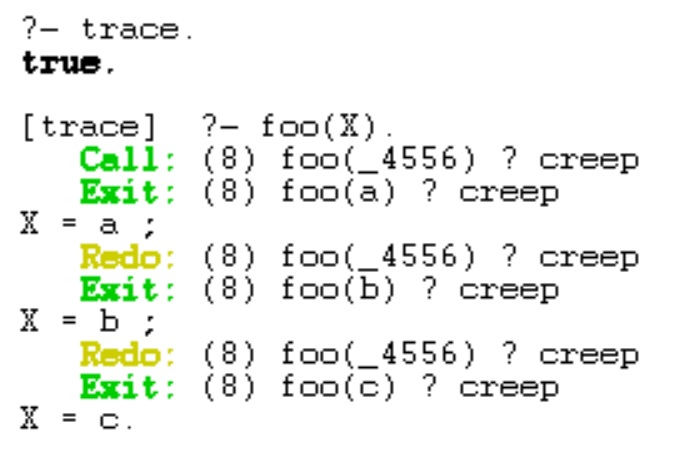
\includegraphics[width=0.4\textwidth]{prolog/trace1}
\end{figure}
\end{multicols}
\end{example}
\end{frame}

%------------------------------------------------------------------

\begin{frame}[fragile]{Cum găsește Prolog răspunsul}

Pentru a găsi un raspuns, \intens{Prolog redenumește variabilele.}

\medskip 
\begin{example}
\begin{multicols}{2}
Să presupunem că avem programul: 
\begin{verbatim}
foo(a). 
foo(b). 
foo(c).
\end{verbatim}
și că punem următoarea întrebare: \\
{\color{blue}\texttt{?- foo(X).}}
\columnbreak
\begin{figure}[h]
    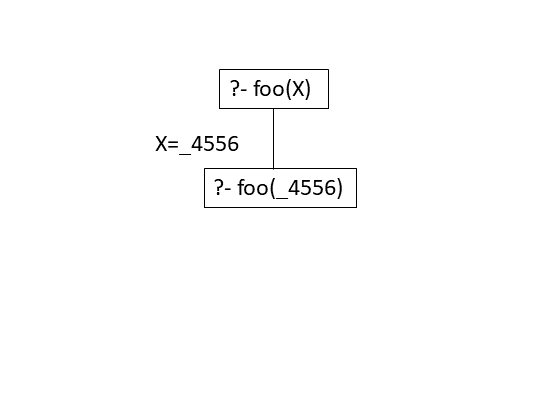
\includegraphics[width=0.4\textwidth]{prolog/foo1}
\end{figure}
\end{multicols}
\end{example}



\end{frame}

\addtocounter{framenumber}{-1}
%------------------------------------------------------------------
\begin{frame}[fragile]{Cum găsește Prolog răspunsul}


Pentru a găsi un raspuns, \intens{Prolog încearcă regulile în ordinea apariției lor.}

\medskip
\begin{example}
\begin{multicols}{2}
Să presupunem că avem programul: 
\begin{verbatim}
foo(a). 
foo(b). 
foo(c).
\end{verbatim}
și că punem următoarea întrebare: \\
{\color{blue}\texttt{?- foo(X).}}
\columnbreak
\begin{figure}[h]
    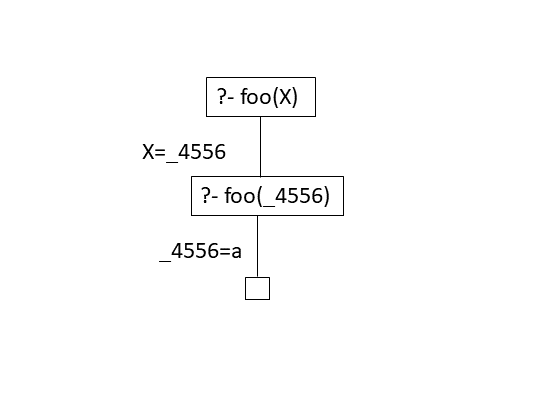
\includegraphics[width=0.4\textwidth]{prolog/foo2}
\end{figure}
\end{multicols}
\end{example}
\medskip

\^{I}n acest moment, a fost găsită  prima soluție: \texttt{X=\_4556=a}.
\end{frame}

\addtocounter{framenumber}{-1}
%------------------------------------------------------------------
\begin{frame}[fragile]{Cum găsește Prolog răspunsul}

Pentru a găsi un raspuns, \intens{Prolog încearcă clauzele în ordinea apariției lor.}

\medskip
\begin{example}
\begin{multicols}{2}
Să presupunem că avem programul: 
\begin{verbatim}
foo(a). 
foo(b). 
foo(c).
\end{verbatim}
și că punem următoarea întrebare: \\
{\color{blue}\texttt{?- foo(X).}}
\columnbreak
\begin{figure}[h]
    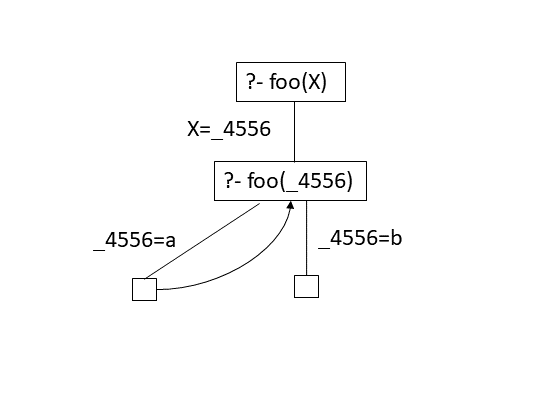
\includegraphics[width=0.4\textwidth]{prolog/foo3}
\end{figure}
\end{multicols}
\end{example}
\medskip

Dacă se dorește încă un răspuns, atunci se face un pas înapoi în \intens{arborele de căutare} și se încearcă satisfacerea țintei cu o nouă valoare.
\end{frame}

\addtocounter{framenumber}{-1}
%------------------------------------------------------------------
\begin{frame}[fragile]{Cum găsește Prolog răspunsul}

Pentru a găsi un raspuns, \intens{Prolog încearcă clauzele în ordinea apariției lor.}

\medskip
\begin{example}
\begin{multicols}{2}
Să presupunem că avem programul: 
\begin{verbatim}
foo(a). 
foo(b). 
foo(c).
\end{verbatim}
și că punem următoarea întrebare: \\
{\color{blue}\texttt{?- foo(X).}}
\columnbreak
\begin{figure}[h]
    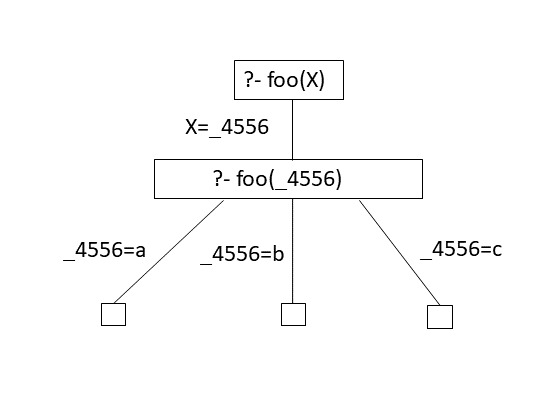
\includegraphics[width=0.4\textwidth]{prolog/foo4}

\begin{center}
\intens{arborele de căutare}
\end{center}
\end{figure}
\end{multicols}
\end{example}

\end{frame}


%-------------------------------------------------------------------

%------------------------------------------------------------------
\begin{frame}[fragile]{Cum găsește Prolog răspunsul}

\medskip 

\begin{example}
\begin{multicols}{2}
Să presupunem că avem programul: 
\begin{verbatim}
bar(b). 
bar(c). 

baz(c).
\end{verbatim}
și că punem următoarea întrebare: \\
{\color{blue}\texttt{?- bar(X),baz(X).}}
\columnbreak
\begin{figure}[h]
    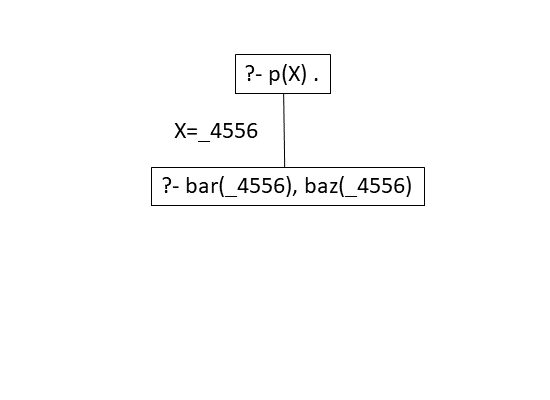
\includegraphics[width=0.4\textwidth]{prolog/bar1}
\end{figure}
\end{multicols}
\end{example}
\end{frame}

\addtocounter{framenumber}{-1}
%------------------------------------------------------------------
\begin{frame}[fragile]{Cum găsește Prolog răspunsul}

\medskip
\intens{Prolog se întoarce la ultima alegere dacă o sub-țintă eșuează.}

\medskip
\begin{example}
\begin{multicols}{2}
Să presupunem că avem programul: 
\begin{verbatim}
bar(b). 
bar(c). 
baz(c).
\end{verbatim}
și că punem următoarea întrebare: \\
{\color{blue}\texttt{?- bar(X),baz(X).}}
\columnbreak
\begin{figure}[h]
    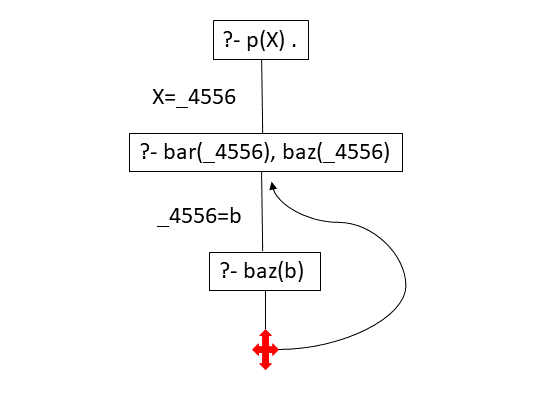
\includegraphics[width=0.4\textwidth]{prolog/bar2}
\end{figure}
\end{multicols}
\end{example}
\end{frame}

\addtocounter{framenumber}{-1}
%------------------------------------------------------------------
\begin{frame}[fragile]{Cum găsește Prolog răspunsul}

\medskip
\intens{Prolog se întoarce la ultima alegere dacă o sub-țintă eșuează.}

\medskip
\begin{example}
\begin{multicols}{2}
Să presupunem că avem programul: 
\begin{verbatim}
bar(b). 
bar(c). 
baz(c).
\end{verbatim}
și că punem următoarea întrebare: \\
{\color{blue}\texttt{?- bar(X),baz(X).}}
\columnbreak
\begin{figure}[h]
    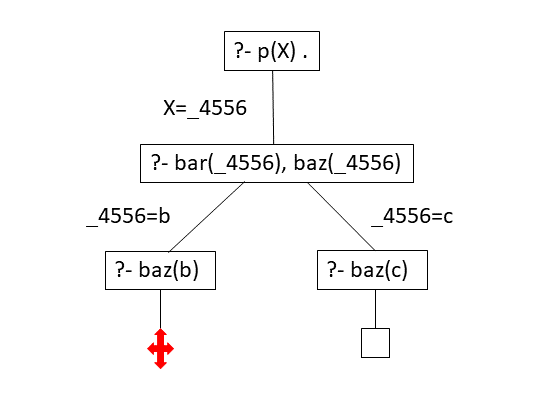
\includegraphics[width=0.4\textwidth]{prolog/bar3}
\end{figure}
\end{multicols}
\end{example}
\medskip

Soluția găsită este: \texttt{X=\_4556=c}.
\end{frame}

%--------------------------------------------------------------

\begin{frame}[fragile]{Cum găsește Prolog răspunsul}

\medskip
Ce se întâmplă dacă schimbăm ordinea regulilor?

\medskip
\begin{example}
\begin{multicols}{2}
Să presupunem că avem programul: 
\begin{verbatim}
bar(c). 
bar(b). 

baz(c).
\end{verbatim}
și că punem următoarea întrebare: \\
{\color{blue}\texttt{?- bar(X),baz(X).}}
\columnbreak
\vspace*{0.3cm}
\end{multicols}
\end{example}
\medskip


\end{frame}


\addtocounter{framenumber}{-1}
%--------------------------------------------------------------

\begin{frame}[fragile]{Cum găsește Prolog răspunsul}

\medskip
Ce se întâmplă dacă schimbăm ordinea regulilor?

\medskip
\begin{example}

Să presupunem că avem programul: 
\begin{verbatim}
bar(c). 
bar(b). 

baz(c).
\end{verbatim}
și că punem următoarea întrebare: \\
{\color{blue}\texttt{?- bar(X),baz(X).}}\\
{\color{blue}\texttt{X = c ;}}\\
{\color{red}\texttt{false}}

\end{example}
\medskip

Vă explicați ce s-a întâmplat? Desenați arborele de căutare!

\end{frame}

%------------------------------------------------------------------
\begin{frame}[fragile]{Un program mai complicat}
\vspace*{0.5cm}

\intens{Problema colorării hărților}
\smallskip

{\em Să se coloreze o hartă dată cu un număr minim de culori astfel încât oricare două țări vecine să fie colorate diferit.}  

\medskip
 \onslide<2-3>{\intens{Cum modelăm această problemă în Prolog?}}
 
\begin{example}
\begin{multicols}{2}
\onslide<3>{
Trebuie să definim:
\begin{itemize}
\item culorile
\item harta
\item constrângerile
\end{itemize}}
\columnbreak
\begin{figure}[h]
    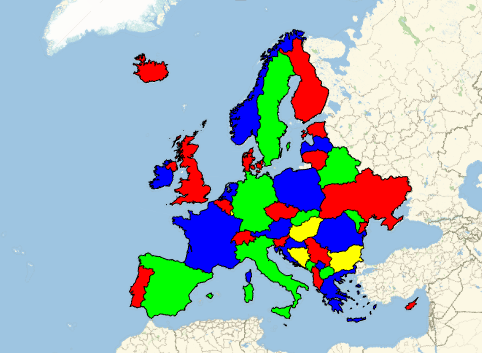
\includegraphics[width=0.4\textwidth]{img/europe1}
    
    \href{https://www.wolfram.com/mathematica/new-in-10/entity-based-geocomputation/find-the-shortest-route-through-the-worlds-capital.html}{\footnotesize{\intens{Sursa imaginii}}}
\end{figure}
\end{multicols}
\end{example}

\end{frame}

\setbeamercolor*{block title}{fg=white, bg=MedianLightOrange}

\addtocounter{framenumber}{-1}
%------------------------------------------------------------------
\begin{frame}[fragile]{Problema colorării hărților}

 \intens{Definim culorile}

\begin{example}
\vspace{-.3cm}
\begin{verbatim}
culoare(albastru).
culoare(rosu).
culoare(verde).
culoare(galben).

\end{verbatim}



\vspace{2.8cm}
\end{example}


\end{frame}

%---------------------------------------------------------------------




\addtocounter{framenumber}{-1}
%%------------------------------------------------------------------

%------------------------------------------------------------------
\begin{frame}[fragile]{Problema colorării hărților}

 \intens{Definim culorile, harta}

\begin{example}
\vspace{-.3cm}
\begin{verbatim}
culoare(albastru).
culoare(rosu).
culoare(verde).
culoare(galben).
\end{verbatim}

\begin{verbatim}
harta(RO,SE,MD,UA,BG,HU) :- vecin(RO,SE), vecin(RO,UA), 
                            vecin(RO,MD), vecin(RO,BG),                      	                         
                            vecin(RO,HU), vecin(UA,MD),
                            vecin(BG,SE), vecin(SE,HU).

                             
\end{verbatim}

\vspace{.4cm}
\end{example}
\end{frame}

\addtocounter{framenumber}{-1}
%------------------------------------------------------------------
\begin{frame}[fragile]{Problema colorării hărților}

\vspace{.4cm}
 \intens{Definim culorile, harta și constrângerile.}
 \onslide<2->{\intens{Cum punem întrebarea?}}


\begin{example}

\vspace{-.3cm}
\begin{verbatim}
culoare(albastru).
culoare(rosu).
culoare(verde).
culoare(galben).
\end{verbatim}

\begin{verbatim}
harta(RO,SE,MD,UA,BG,HU) :- vecin(RO,SE), vecin(RO,UA), 
                            vecin(RO,MD), vecin(RO,BG),                      	                          
                            vecin(RO,HU), vecin(UA,MD),
                            vecin(BG,SE), vecin(SE,HU).
vecin(X,Y) :- culoare(X), 
              culoare(Y), 
              X \== Y.                      
\end{verbatim}
\onslide<3->{\color{blue}\texttt{?- harta(RO,SE,MD,UA,BG,HU).}}
\end{example}
\end{frame}


\addtocounter{framenumber}{-1}
%------------------------------------------------------------------
\begin{frame}[fragile]{Problema colorării hărților}

\vspace{.4cm}
\intens{Ce răspuns primim?}

\begin{example}
\vspace{-.3cm}
\begin{verbatim}
culoare(albastru).
culoare(rosu).
culoare(verde).
culoare(galben).
\end{verbatim}

\vspace{-.3cm}
\begin{verbatim}
harta(RO,SE,MD,UA,BG,HU) :- vecin(RO,SE), vecin(RO,UA), 
                            vecin(RO,MD), vecin(RO,BG),                      	                         
                            vecin(RO,HU), vecin(UA,MD),
                            vecin(BG,SE), vecin(SE,HU).
vecin(X,Y) :- culoare(X), 
              culoare(Y), 
              X \== Y.                      
\end{verbatim}

{\color{blue}\texttt{?- harta(RO,SE,MD,UA,BG,HU).}}


\end{example}

\end{frame}

\addtocounter{framenumber}{-1}
%------------------------------------------------------------------
\begin{frame}[fragile]{Problema colorării hărților}

\bigskip

\begin{example}
\vspace{-.3cm}
\begin{verbatim}
culoare(albastru).
culoare(rosu).
culoare(verde).
culoare(galben).
harta(RO,SE,MD,UA,BG,HU) :-   vecin(RO,SE), vecin(RO,UA), 
                              vecin(RO,MD), vecin(RO,BG),                      	                          
                              vecin(RO,HU), vecin(UA,MD),
                              vecin(BG,SE), vecin(SE,HU).
vecin(X,Y) :- culoare(X), 
              culoare(Y), 
              X \== Y.                      
\end{verbatim}

\vspace{-.2cm}
{\color{blue}\texttt{?- harta(RO,SE,MD,UA,BG,HU).\\
RO = albastru,\\
SE = UA, UA = rosu,\\
MD = BG, BG = HU, HU = verde}} \rule{0.6ex}{1.3ex}

\end{example}

\end{frame}

%---------------------------------------------------------------------
\begin{frame}{Compararea termenilor: \texttt{=},\texttt{\textbackslash=},
\texttt{==},\texttt{\textbackslash==}}
\medskip

\begin{center}
\begin{tabular}{cl}
\intens{\texttt{T = U}} & reușește dacă există  o potrivire 
               (termenii se unifică)\\
\intens{\texttt{T \textbackslash= U}} & reușește dacă nu există o potrivire\\
\intens{\texttt{T == U}} &  reușește dacă termenii sunt identici \\
\intens{\texttt{T \textbackslash== U}} &  reușește dacă termenii sunt diferiți 
              \end{tabular}
              \end{center}
\pause
\begin{example}
\vspace*{-0.2cm}
\begin{alltt}
\begin{tabular}{ll}
?- X = Y.  & ?- X == Y .   \\
X = Y. & \textcolor{red}{false} \\[0.2cm]
?- p(X,q(Z)) = p(Y,X). & ?- p(X,Y) == p(X,Y).   \\
X = Y, Y = q(Z). & \textcolor{red}{true}  \\[0.2cm]
?- 2 = 1 + 1 & ?- 2 == 1 + 1  \\
\textcolor{red}{false} & \textcolor{red}{false}  
\end{tabular}
\end{alltt}
\vspace*{-0.2cm}
\end{example}

\begin{itemize}
\item \^{I}n exemplul de mai sus, \intens{\texttt{1+1}} este privită ca o expresie, nu este evaluată. Există și  predicate care forțează evaluarea. 
\end{itemize}
\end{frame}

%---------------------------------------------------------------------
\begin{frame}[fragile]{Negarea unui predicat: \textcolor{purple}{\texttt{\textbackslash + pred(X)}}}
\vspace*{0.3cm}
\begin{example}
\begin{verbatim}
animal(dog). animal(elephant). animal(sheep).

?- animal(cat).
false
?- \+ animal(cat).
true
\end{verbatim}
\end{example}
\pause

\begin{itemize}
	\item Clauzele din Prolog dau doar condiții suficiente, dar nu și necesare pentru ca un predicat să fie adevărat.
	\item Pentru a da un răspuns pozitiv la o țintă, Prolog trebuie să construiască o "demonstrație" pentru a arată că mulțimea de fapte și reguli din program implică acea țintă.
	\item Astfel, un răspuns \alert{\texttt{false}} nu înseamnă neapărat că ținta nu este adevărată, ci doar că \alert{Prolog nu a reușit să găsească o demonstrație}.	
%		\item Totuși, dacă  \intens{specificăm complet o problemă} (adică specificăm toate cazurile posibile), atunci noțiunile de nedemonstrabil și fals coincid. Atunci un \texttt{false} e chiar un fals.
\end{itemize}
\end{frame}

%---------------------------------------------------------------------
\begin{frame}[fragile]{Operatorul \textcolor{purple}{\textbackslash +}}

\begin{itemize}
	\item  Negarea unei ținte se poate defini astfel:
	
	\begin{verbatim}
    neg(Goal) :- Goal, !, fail.
    neg(Goal)
	\end{verbatim}

unde  \alert{\texttt{fail/0}} este un predicat care eșuează întotdeauna.
\pause
\item \^{I}n PROLOG acest predicat este predefinit sub numele {\texttt {\textbackslash +}}. 
\item Operatorul  \texttt{\textbackslash +} se foloseste pentru a nega un predicat.
	\item \intens{\texttt{!}(cut)} este un predicat predefinit (de aritate 0) care restricționează mecanismul de backtracking:   execuția subțintei \texttt{!} se termină  cu succes, deci alegerile (instanțierile) făcute  înaite de a se ajunge la \texttt{{!}}  nu mai pot fi schimbate.
	
\item O țintă \texttt{\textbackslash + Goal} reușește dacă Prolog nu găsește o demonstrație pentru \texttt{Goal}. Negația din Prolog este definită ca incapacitatea de a găsi o demonstrație.

	\item Semantica operatorului \texttt{{\textbackslash +}} se numește \textcolor{purple}{negation as failure}.

\end{itemize}


\end{frame}

%---------------------------------------------------------------------
\begin{frame}[fragile]{Negația ca eșec ("negation as failure")}

\begin{example}
Să presupunem că avem o listă de fapte cu perechi de oameni căsătoriți între ei:

\begin{verbatim}
married(peter, lucy).
married(paul, mary).
married(bob, juliet).
married(harry, geraldine).
\end{verbatim}
\end{example}
\end{frame}

%---------------------------------------------------------------------
\begin{frame}[fragile]{Negația ca eșec}

\begin{example}[cont.]
Putem să definim un predicat \texttt{\intens{single/1}} care reușește dacă argumentul său nu este nici primul nici al doilea argument în faptele pentru \texttt{married}.

\begin{verbatim}
single(Person) :-
       \+ married(Person, _),
       \+ married(_, Person).
\end{verbatim}

\begin{tabular}{lll}
\texttt{?- single(mary).} &  \texttt{?- single(anne).}  &  \texttt{?- single(X).} \\
\texttt{false}  & \texttt{true} & \texttt{false}
\end{tabular}

\bigskip
Răspunsul la întrebarea \texttt{?- single(anne).} trebuie gândit astfel:
\begin{center}
{\em Presupunem că Anne este single, \\ deoarece \intens{nu am putut demonstra} că este maritată.}
\end{center}
\end{example}
\end{frame}


\begin{frame}[fragile]{Predicatul \texttt{->} /2 (\texttt{if-then-else})}

\begin{itemize}
	\item  \texttt{if-then}
	
	\begin{verbatim}
     If -> Then :- If, !, Then.
	\end{verbatim}
	\pause
	
	\item  \texttt{if-then-else}
	
	\begin{verbatim}
    If -> Then; _Else :- If, !, Then.
    If -> Then; Else :- !, Else.
	\end{verbatim}
	
Se încearcă demonstrarea predicatului \texttt{If}. Dacă întoarce true atunci se încearcă demonstrarea predicatului \texttt{Then}, iar dacă întoarce false se încearcă demonstrarea predicatului \texttt{Else}.	
\end{itemize}

\begin{verbatim}
max(X,Y,Z) :- (X =< Y) -> Z = Y ;  Z = X  
\end{verbatim}

\begin{alltt}
?- max(2,3,Z).
Z = 3.
\end{alltt}

\medskip\pause

Observăm că  \texttt{If -> Then} este  echivalent cu 
\texttt{If -> Then ; fail}.
\end{frame}


%-------------------------------------------------------------
\section{Tipuri de date compuse} \sectionframe
%-------------------------------------------------------------
\begin{frame}{Termeni compuși \texttt{f(t1,$\ldots$, tn)}}
\begin{itemize}
	\item \intens{Termenii} sunt unitățile de bază prin care Prolog reprezintă datele.
	\smallskip
	\item Sunt de 3 tipuri:
	\begin{itemize}
		\smallskip
		\item \intens{Constante}:
		 \texttt{23, sansa, 'Jon Snow'}
		\smallskip
		\item \intens{Variabile}: \texttt{X, Stark, \_house}
		\smallskip
		\item \intens{Termeni compuși:}
\begin{itemize}
\item predicate
\item termeni prin care reprezentăm datele 		\end{itemize}
\end{itemize}
\end{itemize}
\begin{example}
\begin{itemize}
\item \texttt{born(john, date(20,3,1977))}
\begin{itemize}
\item \texttt{born/2} și \texttt{date/3} sunt {\em functori}
\item \texttt{born/2} este un predicat
\item \texttt{date/3} definește  date compuse 
\end{itemize}

\end{itemize}
\end{example}
\end{frame}


\begin{frame}{Tipuri de date definite recursiv}
\begin{itemize}
\item Am văzut că listele sunt definite recursiv astfel:
\medskip

\begin{itemize}
\item \texttt{[]} este listă
\item \texttt{[X|L]} este listă, unde \texttt{X} este element și \texttt{L} este listă
\end{itemize}

\bigskip\pause

\item Cum definim arborii binari în Prolog? \pause Soluție posibilă:\pause
\medskip

\begin{itemize}
\item \texttt{void} este arbore \pause
\item \texttt{tree(X,A1,A2)} este arbore, unde \texttt{X} este un element, iar \texttt{A1} și \texttt{A2} sunt arbori
\end{itemize} 
\end{itemize}
\pause

\begin{center}
\intens{\texttt{tree(X,A1,A2)}} este un termen compus, dar nu este un predicat!
\end{center}
\end{frame}

\begin{frame}{Arbori binari în Prolog}

\begin{itemize}
\item Cum arată un arbore? \pause

\begin{center}
\mbox{\intens{tree(a, tree(b, tree(d, void, void), void), tree(c, void, tree(e, void, void)))}}
\end{center}

\bigskip\pause

\item Cum dăm un "nume" arborelui de mai sus?\pause   \quad Definim un predicat:

\begin{alltt}


\intens{def(arb, tree(a, tree(b,\\
      \hspace*{4.5cm}                   tree(d,void,void),\\
       \hspace*{4.5cm}                  void),\\
       \hspace*{3cm}          tree(c, void,\\
        \hspace*{4.5cm}                 tree(e,void,void)))).}
\end{alltt}
\end{itemize}
\pause
\medskip

 Deoarece în  Prolog nu avem  declarații explicite de date, pentru a defini arborii vom scrie un predicat care este adevărat atunci când argumentul 
său este un arbore.
\end{frame}


\begin{frame}{Arbori binari în Prolog}
\medskip

\begin{itemize}
\item Scrieți un predicat care verifică că un termen este arbore binar. 
\end{itemize}

\pause\medskip

\begin{alltt}
binary\_tree(void).\\
binary\_tree(tree(Element,Left,Right)) :- binary\_tree(Left),

\hspace*{7cm} binary\_tree(Right).
\end{alltt}

\pause
Eventual putem defini și un predicat pentru elemente:

\begin{alltt}
binary\_tree(void).\\
binary\_tree(tree(Element,Left,Right)) :-  binary\_tree(Left), 

\hspace*{6.5cm} binary\_tree(Right), 

\hspace*{6.5cm} element\_binary\_tree(Element).

element\_binary\_tree(X):- integer(X). /* de exemplu */\\

\pause

test:- def(arb,T), binary\_tree(T). 

\end{alltt}
\end{frame}

\begin{frame}{Arbori binari în Prolog}
\begin{block}{Exercițiu}

Scrieți un predicat  care verifică că un element aparține unui arbore.
\medskip

\begin{alltt}
tree\_member(X,tree(X,Left,Right)).

\medskip

	tree\_member(X,tree(Y,Left,Right)) :- tree\_member(X,Left).
	
	\medskip
	
	tree\_member(X,tree(Y,Left,Right)) :- tree\_member(X,Right).
\end{alltt}
\end{block}
\end{frame}


%\begin{frame}{Arbori binari în Prolog}
%\begin{block}{Exercițiu}
%
%Scrieți un predicat  care verifică că  doi arbori binari sunt izomorfi (fiecare nod are acceași copii, dar ordinea nu contează).
%
%\bigskip\pause
%\begin{alltt}
%isotree(void,void).\\
%\medskip
%
%isotree(tree(X,Left1,Right1),tree(X,Left2,Right2)) :- 
%
%	\hfill	isotree(Left1,Left2), isotree(Right1,Right2).
%
%\medskip
%
%	isotree(tree(X,Left1,Right1),tree(X,Left2,Right2)) :- 
%
%\hfill isotree(Left1,Right2), isotree(Right1,Left2).
%\end{alltt}
%\end{block}
%\end{frame}


\begin{frame}{Arbori binari în Prolog}
\begin{block}{Exercițiu}

Scrieți un predicat  care determină parcurgerea în preordine a unui arbore binar. 
\bigskip


\begin{alltt}

preorder(tree(X,L,R),Xs) :-	 preorder(L,Ls),

\hspace*{5cm} preorder(R,Rs), 

\hspace*{5cm}		append([X|Ls],Rs,Xs).\pause

preorder(void,[]).

\pause

test(Tree,Pre):- def(arb, Tree), preorder(Tree,Pre).
\medskip
\pause 

?- test(T,P).\\
T = tree(a, tree(b, tree(d, void, void), void), tree(c, void, tree(e, void, void))),\\
P = [a, b, d, c, e]
\end{alltt}
\end{block}


\end{frame}

%-------------------------------------------------------------
\section{Liste și recursie} \sectionframe
%-------------------------------------------------------------
\begin{frame}{Listă \texttt{[t1,\ldots,tn]}}
\begin{itemize}
\item O listă în Prolog este un șir de elemente, separate prin virgulă, între paranteze drepte:

\begin{center}
\intens{\texttt{[1,cold, parent(jon),[winter,is,coming],X]}}
\end{center}
\item O listă poate conține termeni de orice fel.
\item Ordinea termenilor din listă are importanță:
\begin{alltt}
?- [1,2] == [2,1] .\\
\alert{false}
\end{alltt}
\item Lista vidă se notează \intens{[$ \, $]}.
\item Simbolul \intens{$\mid$} delimitează coada listei:
\begin{alltt}
?- [1,2,3,4,5,6] = [X|T]. \\
X = 1, T = [2, 3, 4, 5, 6].\\
\medskip
?- [1,2,3|[4,5,6]] == [1,2,3,4,5,6].\\
true.
\end{alltt}
\end{itemize}
\end{frame}

\begin{frame}{Listă \texttt{[t1,\ldots,tn]==[t1 |[t2,\ldots,tn]}}
\begin{itemize}
\item Simbolul \intens{$\mid$} delimitează coada listei:
\begin{alltt}
?- [1,2,3,4,5,6] = [X|T]. \\
X = 1, \\
T = [2, 3, 4, 5, 6].
\end{alltt}

\item Variabila anonimă \intens{\texttt{\_}} este unificată cu orice termen Prolog:
\begin{alltt}
?- [1,2,3,4,5,6] = [X|\_]. \\
X = 1.
\end{alltt}

\item Deoarece Prologul face unificare poate identifica șabloane mai complicate: 
\begin{alltt}
?- [5,1,1,3,2]=[\_|[X|[X|\_]]].\\
X = 1.

?- [5,1,4,3,2]=[\_|[X|[X|\_]]].\\
false.
\end{alltt}
\end{itemize}
\end{frame}

\begin{frame}{Liste}
\vspace*{0.5cm}

\begin{block}{Exercițiu}
\begin{itemize}
\item Definiți un predicat care verifică că un termen este lista.

\begin{alltt}
is\_list([]).\\
is\_list([\_|\_]).
\end{alltt}
\pause

\item Definiți predicate care verifică dacă un termen este  primul element, ultimul element sau coada unei liste.
\vspace*{0.2cm}

\begin{alltt}
head([X|\_],X). \\

last([X],X). \\
last([\_|T],Y):- last(T,Y).\\
 
tail([],[]).\\
tail([\_|T],T).
\end{alltt}
\end{itemize}
\end{block}



\end{frame}

\begin{frame}{Liste}
\vspace*{0.3cm}

\begin{block}{Exercițiu}
\begin{itemize}
\item Definiți un predicat care verifică dacă un termen aparține unei liste.

\begin{alltt}
member(H, [H|\_]).\\
member(H, [\_|T]) :- member(H,T).
\end{alltt}


\medskip\pause

\item Definiți un predicat \texttt{append/3} care verifică dacă o listă se obține prin concatenarea altor două liste.

\begin{alltt}
append([],L,L).\\
append([X|T],L, [X|R]) :- append(T,L,R).\\
\end{alltt}

\end{itemize}
\end{block}

\pause
Există predicatele predefinite \intens{\texttt{member/2}} și 
\intens{\texttt{append/3}}. 
\end{frame}

\begin{frame}{Liste \texttt{append/3}}

\vspace*{0.3cm}

\begin{itemize}
\item Funcția \texttt{append/3}:
\begin{alltt}
?- listing(append/3).\\
append([],L,L).\\
append([X|T],L, [X|R]) :- append(T,L,R).\\

?- append(X,Y,[a,b,c]).\\
X = [],\\
Y = [a, b, c] ;\\
X = [a],\\
Y = [b, c] ;\\
X = [a, b],\\
Y = [c] ;\\
X = [a, b, c],\\
Y = [] ;\\
\alert{false}
\end{alltt}
\item Funcția astfel definită poate fi folosită 
atât pentru verificare, cât și pentru generare. 
\end{itemize}


\end{frame}

\begin{frame}{Liste}
\vspace*{0.3cm}

\begin{block}{Exercițiu}
\begin{itemize}
\item Definiți un predicat \texttt{elim/3} care verifică dacă o  listă se obține din alta prin eliminarea unui element.
\medskip\pause
\begin{alltt}
elim(X, [X|T], T).\\
elim(X, [H|T], [H|L]) :- elim(X,T,L).
\end{alltt}


\medskip\pause

\item Definiți un predicat care \texttt{perm/2} care verifică dacă două liste sunt permutări.
\medskip\pause
\begin{alltt}
perm([],[]).
perm([X|T],L) :- elim(X,L,R), perm(R,T).
\end{alltt}

\end{itemize}
\end{block}
\pause
Predicatele predefinite \intens{\texttt{select/3}} și 
\intens{\texttt{permutation/2}} au aceeași funcționalitate. 
\end{frame}

\begin{frame}{Generează și testează}
\vspace*{0.3cm}

\begin{center}
\intens{\texttt{solution(X) :- generate(X), check(X).}}
\end{center}

\begin{block}{Exercițiu}
Determinați toate cuvintele dintr-o bază de 
cunoștințe dată, care sunt anagrame ale unui cuvânt dat.

\medskip

KB: \texttt{word(relay). word(early). word(layer).}
\medskip

Predicat util:\\
\begin{alltt}
?- name(relay,L). \% {\em conversie între atomi și liste}\\
L = [114, 101, 108, 97, 121]
\end{alltt}
\end{block}
\pause
Două abordări posibile:
\begin{itemize}
\item  se generează o posibilă, soluție apoi se testează dacă este în KB.
\item se parcurge KB și pentru fiecare termen se testează dacă e soluție. 
\end{itemize}
\end{frame}

\begin{frame}{Generează și testează}
\vspace*{0.3cm}

\begin{center}
\intens{\texttt{solution(X) :- generate(X), check(X).}}
\end{center}

\begin{block}{Exercițiu}
Determinați toate cuvintele dintr-o bază de 
cunoștințe dată, care sunt anagrame ale unui
 cuvânt dat.
\medskip

KB: \texttt{word(relay). word(early). word(layer).}
\medskip

\pause
\begin{alltt}
anagram1(A,B) :- name(A,L), permutation(L,W), \\
\hspace*{3cm} name(B,W), word(B).\\ \pause
anagram2(A,B) :-  name(A,L), word(B), \\
\hspace*{3cm} name(B,W),  permutation(L,W).\\
\end{alltt}
\pause

\begin{columns}
\begin{column}{0.45\textwidth}
\begin{alltt}
?- anagram1(layre,X).\\
X = layer ;\\
X = relay ;\\
X = early ;\\
\alert{false.}
\end{alltt}
\end{column}
\begin{column}{0.45\textwidth}
\begin{alltt}
?- anagram2(layre,X).\\
X = relay ;\\
X = early ;\\
X = layer ;\\
\alert{false.}
\end{alltt}
\end{column}
\end{columns}
\end{block}
\end{frame}


\begin{frame}{Recursie}
\vspace*{0.3cm}

\begin{block}{Exercițiu}
\begin{itemize}

\item Definiți un predicat \texttt{rev/2} care verifică dacă o listă este inversa altei liste. 
\medskip\pause
\begin{alltt}
rev([],[]).\\
rev([X|T],L) :- rev(T,R),append(R,[X],L).
\end{alltt}
\end{itemize}
\end{block}

Soluția de mai sus este corectă, dar foarte costisitoare computațional, datorită stilului de programare declarativ. 
\medskip


\intens{Cum putem defini o variantă mai rapidă?}

\medskip

O metodă care prin care recursia devine mai rapidă este folosirea \intens{acumulatorilor}, în care se păstrează rezultatele parțiale.
 
\end{frame}

\begin{frame}{Recursie cu acumulatori}
\begin{itemize}
\item Varianta inițială:
\begin{alltt}
rev([],[]).\\
rev([X|T],L) :- rev(T,R),append(R,[X],L). 
\end{alltt}
\item Varianta cu acumulator
\begin{alltt}
rev(L,R) :- revac(L,\intens{[]},R).\\
\% {\em la momentul inițial nu am acumulat nimic.  }    
\medskip\pause

revac([], \intens{R}, R).\\
\% {\em cand lista inițială a fost consumată,}\\
\% {\em am acumulat rezultatul final.}
\medskip\pause

revac([X|T], \intens{Acc}, R) :- revac(T,\intens{[X|Acc]},R).\\
\% \texttt{Acc} {\em conține inversa listei care a fost deja parcursă.} 
\end{alltt}
\item Complexitatea a fost redusă de la $O(n^2)$ la $O(n)$, unde $n$ este lungimea listei.
\end{itemize}
\end{frame}

\begin{frame}{Recursie}

\begin{itemize}
\item Multe implementări ale limbajului Prolog aplică "{\em last call optimization}" atunci când un apel recursiv este ultimul predicat din corpul unei clauze ({\em tail recursion}).

\medskip
\item Atunci când este posibil, se recomandă utilizare recursiei la coadă ({\em tail recursion}).

\medskip
\item Vom defini un predicat care generează liste lungi în două moduri și vom analiza performanța folosind predicatul \intens{time/1}.
\end{itemize}

\pause
\begin{alltt}
biglist(0,[]).\\
biglist(N,[N|T]) :- N >= 1, M is N-1,biglist(M,T),M=M.\\

biglist\_tr(0,[]).\\
biglist\_tr(N,[N|T]) :- N >= 1, M is N-1,biglist\_tr(M,T).
\end{alltt}


\end{frame}

\begin{frame}{Recursie la coadă}

\vspace*{0.5cm}

\begin{itemize}
\item Predicat \textcolor{magenta}{fără} recursie la coadă:
\begin{alltt}
biglist(0,[]).\\
biglist(N,[N|T]) :- N >= 1, M is N-1,biglist(M,T),\textcolor{magenta}{M=M}.
\end{alltt}

Apelul recursiv întoarce valoarea găsită în predicatul apelant, acestă valoare urmând a fi prelucrată. \pause

\begin{alltt}
?- time(biglist(50000,X)).\\
\intens{ 100,000 inferences, 0.016 CPU in 0.038 seconds \\
(41\% CPU, 6400000 Lips)}\\
X = [50000, 49999, 49998|...] .
\end{alltt}\pause

\item Predicatul \intens{cu} recursie la coadă:
\begin{alltt}
biglist\_tr(0,[]).\\
biglist\_tr(N,[N|T]) :- N >= 1, M is N-1,biglist\_tr(M,T).\\
\pause

?- time(biglist\_tr(50000,X)).\\
\intens{100,000 inferences, 0.000 CPU in 0.007 seconds \\(0\% CPU, Infinite Lips)}\\
X = [50000, 49999, 49998|...]
\end{alltt} 

\end{itemize}
\end{frame}



%\begin{frame}{Liste}
%\begin{alltt}
%append([],L,L).\\
%append([X|T],L, [X|R]) :- append(T,L,R).\\
%\end{alltt}
%
%
%\begin{block}{Exercițiu}
% Definiți \intens{\texttt{prefix/2}} și \intens{\texttt{suffix/2}} folosind \texttt{append}.
%\pause
%
%\begin{alltt}
%prefix(P,L) :- append(P,\_, L).\\
%suffix(S,L)  :- append(\_,S,L).\\
%\end{alltt} 
%\end{block}
%\pause
%
%Observăm că funcția \texttt{append} parcurge prima listă.
%\medskip
%
%\intens{Am putea rescrie această funcție astfel încât legătura să se facă direct, așa cum putem face în programarea imperativă?}
%
%\medskip\pause
%
%Problema poate fi rezolvată scriind \intens{listele ca diferențe}, o tehnică utilă în limbajul Prolog.
%\end{frame}
%
%\begin{frame}{Liste ca diferențe}
%\begin{itemize}
%\item Ideea:  lista \texttt{[t1,\ldots,tn]} va fi reprezentată printr-o pereche 
%\begin{center}
%\intens{\texttt{([t1,\ldots,tn|T], T)}}
%\end{center}
%
%Această pereche poate fi notată \intens{\texttt{[t1,\ldots,tn|T]- T}}, dar notația nu este importantă. 
%
%\pause
%
%\item Vrem să definim \texttt{append/3} pentru liste ca diferențe:
%
%\medskip
%
%\texttt{\intens{dlappend((X1,T1),(X2,T2),(R,T)) :-} \alert{?}.} 
%
%\end{itemize}
%
%
% 
%\begin{alltt}
%?- dlappend(([1,2,3|P],P),([4,5|T],T),RD).\\
%P = [4, 5|T],\\
%RD =  ([1, 2, 3, 4, 5|T], T).\\
%\end{alltt}
%
%\end{frame}
%
%\begin{frame}{Liste ca diferențe \texttt{([t1,\ldots,tn|T], T)}}
% \medskip
% 
% \texttt{dlappend((X1,T1),(X2,T2),(R,T)) :- \alert{?}.} \\
%
%\pause\medskip
%
%\begin{itemize}
%\item Dacă \texttt{[t1,\ldots, tn]} este diferența \texttt{(X1,T1)}, iar \texttt{[q1,\ldots, qk]} este diferența \texttt{(X2,T2)} observăm că diferența \texttt{(R,T)} trebuie să fie  \texttt{[t1,\ldots,tn,q1\ldots, qk]}. \pause
%\item  Obținem  \texttt{R=[t1,\ldots,tn,q1\ldots, qk|T]}, deci 
%
%\texttt{(X1,T1) = (R, P)}  și  \texttt{(X2,T2) = (P,T)}
%
%unde \texttt{P =[q1,\ldots,qk|T])}.\pause
%
%\item Definiția este:
%\begin{center}
%\texttt{\intens{dlappend((R,P),(P,T),(R,T)).}}
%\end{center}
%\end{itemize}
% 
%\begin{alltt}
%?- dlappend(([1,2,3|P],P),([4,5|T],T),RD).\\
%P = [4, 5|T],\\
%RD =  ([1, 2, 3, 4, 5|T], T).\\
%\end{alltt}
%\pause
%
%\begin{itemize}
%\item \texttt{dlappend} este foarte rapid, dar nu poate fi folosit pentru generare, ci numai pentru verificare. 
%\end{itemize}
%\end{frame}



%-------------------------------------------------------------
\section{Exemplu: reprezentarea unei GIC} \sectionframe
%-------------------------------------------------------------
\begin{frame}[fragile]{Structura frazelor}
\begin{itemize}
 \item  Aristotel, On Interpretation, 
 {\small{\url{http://classics.mit.edu/Aristotle/interpretation.1.1.html}:}}
\begin{center} 
\intens{ "Every affirmation, then, and every denial, will consist of a noun and a verb, either definite or indefinite." }
\end{center} 

 \medskip\pause
 
 \item N. Chomsy, Syntactic structure, Mouton Publishers, First printing 1957 - Fourteenth printing 1985 [Chapter 4 (Phrase Structure)]
 \medskip
\begin{center}
\intens{
\begin{tabular}{l} 
(i) $Sentence \, \to\, NP+ VP$\\
(ii) $ NP \,\to\, T+N$\\
(iii) $VP \,\to\, Verb + NP$\\
(iv) $T\,\to\,the$\\
(q) $N\,\to\, fman, ball,$ etc.\\
(vi) $V\,\to\, hit, took,$ etc.
\end{tabular}}
\end{center}
 \end{itemize}
\end{frame}

\begin{frame}{Gramatică  independentă de context}

\begin{itemize}
\item Definim structura propozițiilor folosind o 
gramatică independentă de context:
\end{itemize}
\bigskip

\begin{columns}
\begin{column}{0.35\textwidth}
\begin{tabular}{lcl}
S &$\to$ & NP VP \\
NP &$\to$ &Det N \\
VP &$\to$ & V\\
VP &$\to$ & V NP\\
Det &$\to$ & $the$\\
Det &$\to$ & $a$\\
N &$\to$ & $boy$\\
N &$\to$ & $girl$\\
V &$\to$ & $loves$\\
V &$\to$ & $hates$ 
\end{tabular}
\end{column}
\begin{column}{0.6\textwidth}
\begin{itemize}
\item Neterminalele definesc categorii gramaticale:
\medskip

S (propozițiile),

NP (expresiile substantivale), 

VP (expresiile verbale),

V (verbele), 

N (substantivele), 

Det (articolele).


\item  Terminalele  definesc cuvintele.
\end{itemize}
\end{column}
\end{columns}
\end{frame}




\begin{frame}{Gramatică  independentă de context}
\begin{block}{GIC}
\begin{columns}
\begin{column}{0.45\textwidth}
\begin{tabular}{lcl}
S &$\to$ & NP VP \\
NP &$\to$ &Det N \\
VP &$\to$ & V\\
VP &$\to$ & V NP\\

\end{tabular}
\end{column}
\begin{column}{0.45\textwidth}
\begin{tabular}{lcl}
Det &$\to$ & $the$\\
Det &$\to$ & $a$\\
N &$\to$ & $boy$\\
N &$\to$ & $girl$\\
V &$\to$ & $loves$\\
V &$\to$ &  $hates$
\end{tabular}
\end{column}
\end{columns}
\end{block}

\intens{Ce vrem să facem?}

\begin{itemize}
\item Vrem să scriem un program în Prolog care să recunoască propozițiile generate de această 
gramatică.
\item  Reprezentăm propozițiile prin  liste.
\end{itemize}
\begin{alltt}
?- atomic\_list\_concat(SL,' ' , 'a boy loves a girl').\\
SL = [a, boy, loves, a, girl]
\end{alltt}
\end{frame}

%--------------------------------------------

\begin{frame}{Definirea unei gramatici în Prolog}
\begin{itemize}
\item  Reprezentăm propozițiile prin  liste.
\begin{alltt}
SL = [a, boy, loves, a, girl]
\end{alltt}
\medskip\pause

\item Fiecărui neterminal îi asociem un predicat care definește listele corespunzătoare categoriei gramaticale respective. 
\medskip
\texttt{n([boy]). n([girl]). det([the]). v([loves]).}
\medskip\pause

\item Lista asociată unei  propoziții se obține prin concatenarea listelor asociate elementelor componente.
\medskip\pause

De exemplu, interpretăm regula \intens{S $\to$  NP VP} astfel:
\medskip

\intens{o propozi\ tie este o listă \texttt{L} care se obține prin concatenarea a două liste,  \texttt{X} și \texttt{Y}, unde \texttt{X} reprezintă o expresie substantivală și \texttt{Y} reprezintă o expresie verbală.} 
\medskip

\texttt{s(L) :- np(X), vp(Y), append(X,Y,L)}.

\end{itemize}

\end{frame}

\begin{frame}{Definirea unei gramatici în Prolog}

\vspace*{0.5cm}

\begin{block}{Gramatică independentă de context}
\begin{columns}
\begin{column}{0.45\textwidth}
\begin{tabular}{lcl}
S &$\to$ & NP VP \\
NP &$\to$ &Det N \\
VP &$\to$ & V\\
VP &$\to$ & V NP\\

\end{tabular}
\end{column}
\begin{column}{0.45\textwidth}
\begin{tabular}{lcl}
Det &$\to$ & $the$\\
Det &$\to$ & $a$\\
N &$\to$ & $boy$\\
N &$\to$ & $girl$\\
V &$\to$ & $loves$\\
V &$\to$ &  $hates$
\end{tabular}
\end{column}
\end{columns}
\end{block}


\begin{block}{Prolog}
\begin{columns}
\begin{column}{0.55\textwidth}
\begin{alltt}
s(L) :- np(X), vp(Y),\\
\hspace*{1.4cm}  append(X,Y,L).\\
np(L) :- det(X), n(Y), \\
\hspace*{1.6cm} append(X,Y,L) .\\
vp(L) :- v(L).\\
vp(L):- v(X), np(Y),\\
\hspace*{1.4cm} append(X,Y,L) .\\
\end{alltt}
\end{column}
\begin{column}{0.35\textwidth}
\begin{alltt}
det([the]).\\ det([a]).\\
n([boy]). \\ n([girl]). \\
v([loves]).\\  v([hates]).
\end{alltt}
\end{column}
\end{columns}
\end{block}
\end{frame}


\begin{frame}{Definirea unei gramatici în Prolog}
\vspace*{0.3cm}

\begin{columns}
\begin{column}{0.45\textwidth}
\begin{alltt}
{
s(L) :- np(X), vp(Y),\\
\hspace*{1.4cm}  append(X,Y,L).\\

np(L) :- det(X), n(Y), \\
\hspace*{1.6cm} append(X,Y,L) .\\

vp(L) :- v(L).\\
vp(L):- v(X), np(Y),\\
\hspace*{1.4cm} append(X,Y,L) .\\

det([the]).\\ det([a]).\\
n([boy]). \\ n([girl]). \\
v([loves]).\\  v([hates]).}
\end{alltt}
\end{column}
\begin{column}{0.45\textwidth}
\begin{alltt}
?- s([a,boy,loves, a, girl]).\\
true .\\
\medskip

?- s[a, girl|T].\\
T = [loves] ;\\
T = [hates] ;\\
T = [loves, the, boy] ;\\
$\vdots$
\medskip

?- s(S).\\
S = [the, boy, loves] ;\\
S = [the, boy, hates] ;\\
$\vdots$
\end{alltt}
\end{column}
\end{columns}

\end{frame}

\begin{frame}{Definirea unei gramatici în Prolog}
\begin{itemize}
\item  Reprezentăm propozițiile prin  liste.
\begin{alltt}
SL = [a, boy, loves, a, girl]
\end{alltt}
\medskip\pause

\item Fiecărui neterminal îi asociem un predicat care definește listele corespunzătoare categoriei gramaticale respective. 
\medskip
\texttt{n([boy]). n([girl]). det([the]). v([loves]).}
\medskip\pause

\item Lista asociată unei  propoziții se obține prin concatenarea listelor asociate elementelor componente.
\medskip\pause


\item Deși corectă, reprezentarea anterioară este ineficientă, arborele de căutare este foarte mare. 
 Pentru a optimiza, folosim {\em reprezentarea listelor ca diferențe}.



\end{itemize}

\end{frame}
%---------------------------------------------------------------------



\begin{frame}{Bibliografie}
\begin{itemize}
		
	\item M. Ben-Ari, \textbf{Mathematical Logic for Computer Science}, Springer, 2012.
	\vspace{.2cm}
	\item P. Blackburn, J. Bos, K. Striegnitz, \textbf{Learn Prolog now}, College Publications, 2006.
	\vspace{.2cm}
	\item J.W. Lloyd, Foundations of Logic Programming, Springer, 1987.
	\vspace{.2cm}
	\item L.S. Sterling and E.Y. Shapiro, The Art of Prolog \url{https://mitpress.mit.edu/books/art-prolog-second-edition}
	\vspace{.2cm}
	\item Logic Programming, The University of Edinburgh, https://www.inf.ed.ac.uk/teaching/courses/lp/
\end{itemize}
\end{frame}
%---------------------------------------------------------------------

\begin{frame}
\begin{center}
\intens{Pe săptămâna viitoare!}
\end{center}
\end{frame}
\end{document}




































